\documentclass[12pt, a4paper]{article}

\usepackage[utf8]{inputenc}
\usepackage{geometry}
\geometry{top=2.5cm, bottom=2.5cm, left=2.5cm, right=2.5cm}
\usepackage{graphicx}
\usepackage{booktabs}
\usepackage{hyperref}
\usepackage{float}
\usepackage{amsmath}

\title{
    \vspace{-2cm}
    \Large \textbf{Assignment 1: Multi-class Diabetes Risk Prediction}
}
\author{
    Mohand Sayed   (22011902) \\
    Ali Eldeen     (22010934) \\
    Youssef Khamis (22011381)
}

\date{}

\begin{document}

\maketitle

\section{Dataset and Preparation}
\subsection{Data Splitting and Random Seed}
To ensure reproducibility, all random operations were initialized with a fixed random seed of 42. The dataset was split into 70\% training, 10\% validation, and 20\% testing using stratified splitting to maintain the original class distribution across all subsets.

\subsection{Feature Preprocessing and Selection}
Numerical features, specifically BMI, MentHlth, PhysHlth, Education, Income and Age, were standardized using a standard scaler to prevent attributes with larger scales from mathematically dominating distance calculations in models like KNN. 

To identify the most predictive features and reduce dimensionality, we applied the Chi-Squared ($\chi^2$) statistical test using a SelectKBest approach. This allowed us to filter the original 21 features down to the 10 most informative attributes, streamlining model efficiency and focusing on the most statistically significant predictors of diabetes risk.

\subsection{Handling Class Imbalance}
The original dataset suffers from severe class imbalance. To mitigate this during training, we explored three techniques: Random Oversampling, SMOTE (Synthetic Minority Over-sampling Technique), and Random Undersampling. Both Random Oversampling and SMOTE successfully balanced the training set by increasing the minority classes to match the majority class, resulting in exactly 133,038 samples per class. SMOTE yielded the best validation performance for our distance-based models.

\section{Implementation Details}
For each of the following models, two versions were trained: a Baseline version on the original imbalanced training set, and a Balanced version using the handled dataset. Hyperparameters were tuned exclusively using the 10\% validation set.

\subsection{K-Nearest Neighbors (KNN)}
During the hyperparameter tuning phase on the validation set, we experimented with k values of 3, 5, 11, and 21, and evaluated both Euclidean and Manhattan distance metrics. For the Baseline model trained on imbalanced data, the optimal configuration was found to be k=5 using the Manhattan distance. For the Balanced model trained on the SMOTE dataset, the best configuration remained k=5 with Manhattan distance (though Random Oversampling favored Euclidean).

\subsection{Softmax Regression}
For Softmax (Multinomial Logistic) Regression, the regularization parameter $C$ was tuned over a logarithmic grid: $\{10^{-4}, 10^{-3}, 10^{-2}, 10^{-1}, 1, 10, 100, 10^{3}, 10^{4}\}$. The model was trained using the \texttt{lbfgs} solver with \texttt{multi\_class=multinomial} and a maximum of 5000 iterations. The optimal $C$ was selected by maximising the \textbf{Macro-F1} score on the validation set, making the selection criterion directly aligned with the primary evaluation metric for this imbalanced dataset.

Beyond the standard balancing strategies (Oversampling, SMOTE, Undersampling, SMOTEENN, and Class Weights), one additional technique was explored:
\begin{itemize}
    \item \textbf{Per-class Threshold Tuning:} Instead of using the default 0.5 decision threshold for all classes, a grid search over thresholds $[0.1, 0.9]$ was performed on the validation set to find the per-class threshold combination that maximises Macro-F1. The best thresholds found were $[0.1, 0.3, 0.3]$ for No Diabetes, Pre-diabetes, and Diabetes respectively.
\end{itemize}

\subsection{Custom Feedforward Neural Network (FNN)}
To benchmark a non-linear model, we implemented a custom Feedforward Neural Network (FNN) for multi-class classification. The network was trained on the same preprocessed feature set used by the linear models, and produced class probabilities through a Softmax output layer. The model was optimised with categorical cross-entropy loss and monitored using early stopping on the validation loss to reduce overfitting.

To address class imbalance, the FNN was trained under multiple data strategies: baseline (no balancing), random oversampling, SMOTE, random undersampling, SMOTEENN, and class-weighted loss. Hyperparameters were tuned on the validation set (with a fixed seed of 42 for all randomised operations).

\section{Evaluation}

\subsection{Metric Justification}
For this specific imbalanced dataset, \textbf{Macro-F1} is the most meaningful and reliable metric. Because the "No Diabetes" class vastly outnumbers the "Prediabetes" class, Accuracy and Micro-F1 are highly misleading; a model can achieve over 80\% accuracy simply by guessing the majority class every time. Macro-F1 calculates the F1-score for each class independently and averages them equally, punishing models that completely fail to identify the minority classes.

\subsection{Results Summary}
Table \ref{tab:results} summarizes the performance of all trained models on the isolated test set.

\begin{table}[H]
    \centering
    \caption{Model Performance Comparison on Test Set}
    \label{tab:results}
    \begin{tabular}{lcccc}
        \toprule
        \textbf{Model Version} & \textbf{Accuracy} & \textbf{Micro-F1} & \textbf{Macro-F1} & \textbf{Weighted-F1} \\
        \midrule
        KNN (Baseline)      & 0.8166 & 0.8166 & 0.3994 & 0.7870 \\
        KNN (SMOTE)         & 0.7177 & 0.7177 & 0.4166 & 0.7453 \\
        KNN (Oversamp.)     & 0.7032 & 0.7032 & 0.4131 & 0.7347 \\
        KNN (Undersamp.)    & 0.5827 & 0.5827 & 0.3987 & 0.6693 \\
        \midrule
        Softmax (Baseline)          & 0.8331 & 0.8331 & 0.3886 & 0.7900 \\
        Softmax (Oversamp.)         & 0.6340 & 0.6340 & 0.4267 & 0.7100 \\
        Softmax (SMOTE)             & 0.6384 & 0.6384 & 0.4276 & 0.7100 \\
        Softmax (Undersamp.)        & 0.6893 & 0.6893 & 0.4323 & 0.7300 \\
        Softmax (SMOTEENN)          & 0.5915 & 0.5915 & 0.4142 & 0.6800 \\
        Softmax (Class Weights)     & 0.6501 & 0.6501 & 0.4310 & 0.7200 \\
        Softmax (Thr. Tuning)       & 0.7783 & 0.7783 & 0.4602 & 0.7900 \\
        \midrule
        FNN (Baseline)              & 0.8380 & 0.8380 & 0.3915 & 0.8380 \\
        FNN (Oversamp.)             & 0.6199 & 0.6199 & 0.4194 & 0.6199 \\
        FNN (SMOTE)                 & 0.6285 & 0.6285 & 0.4186 & 0.6285 \\
        FNN (Undersamp.)            & 0.6631 & 0.6631 & 0.4279 & 0.6631 \\
        FNN (SMOTEENN)              & 0.5694 & 0.5694 & 0.4028 & 0.5694 \\
        FNN (Class Weights)         & 0.6520 & 0.6520 & 0.4243 & 0.6520 \\
        \bottomrule
    \end{tabular}
\end{table}

\subsection{Confusion Matrices}
% Export your Confusion Matrix plots from your Jupyter notebook and uncomment the \includegraphics lines below to display them in a 2x2 grid for each model.

\subsubsection{K-Nearest Neighbors (KNN)}
\begin{figure}[H]
    \centering
    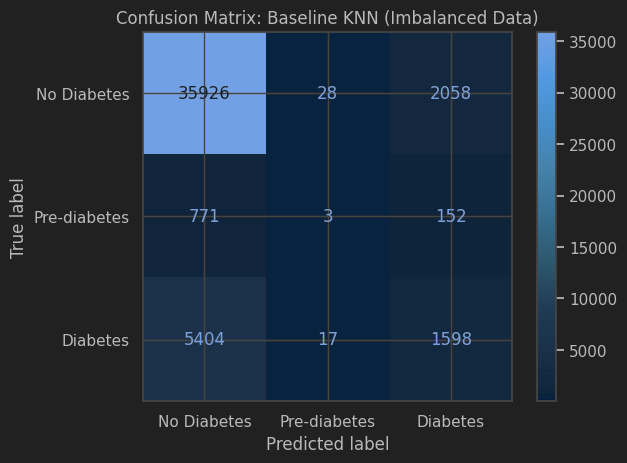
\includegraphics[width=0.45\textwidth]{knn_baseline_cm.png}
    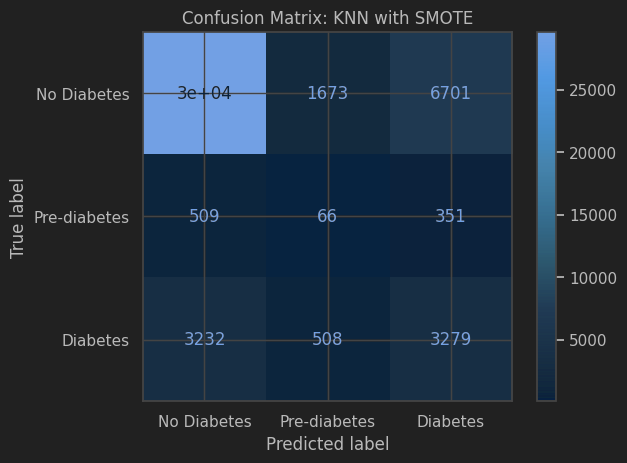
\includegraphics[width=0.45\textwidth]{knn_smote_cm.png} \\
    \vspace{0.5cm}
    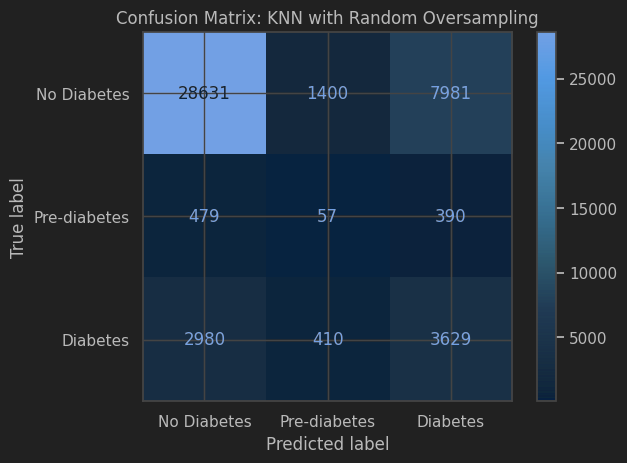
\includegraphics[width=0.45\textwidth]{knn_oversample_cm.png}
    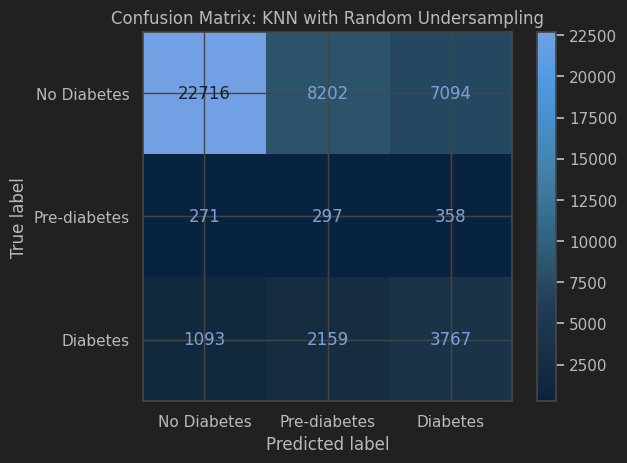
\includegraphics[width=0.45\textwidth]{knn_undersample_cm.png}
    \caption{KNN Confusion Matrices (Top Left: Baseline, Top Right: SMOTE, Bottom Left: Oversampled, Bottom Right: Undersampled)}
\end{figure}

\subsubsection{Softmax Regression}
\begin{figure}[H]
    \centering
    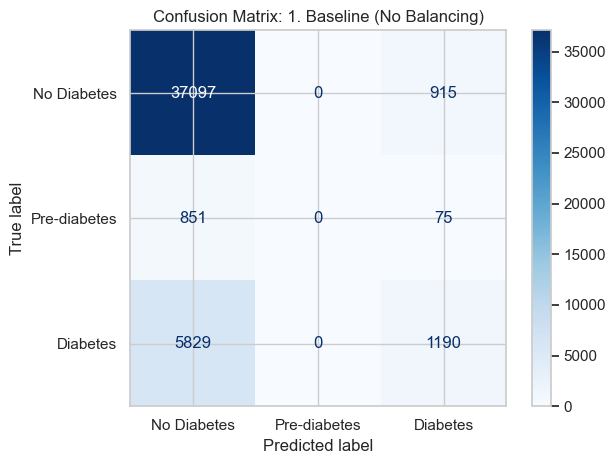
\includegraphics[width=0.45\textwidth]{softmax_baseline_cm.png}
    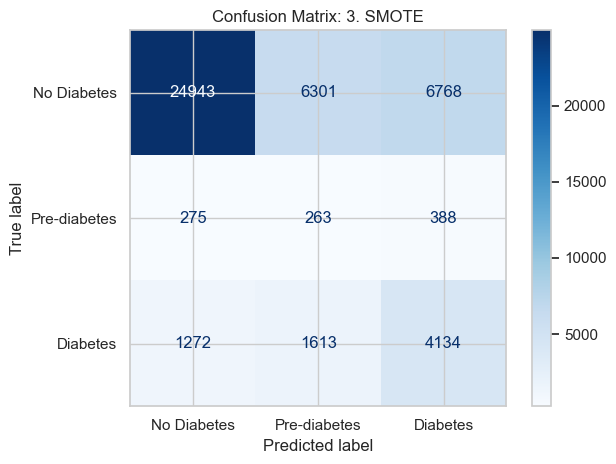
\includegraphics[width=0.45\textwidth]{softmax_smote_cm.png} \\
    \vspace{0.3cm}
    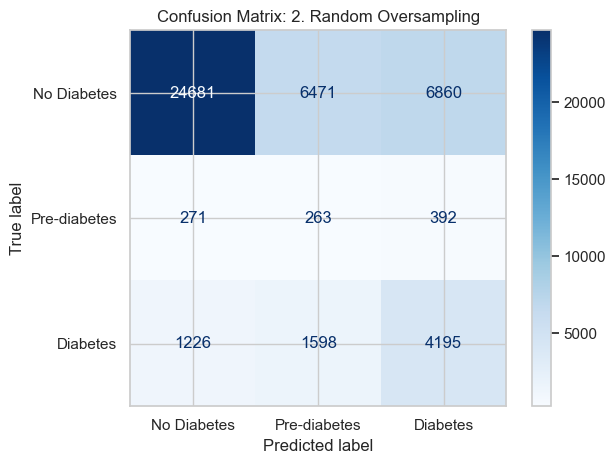
\includegraphics[width=0.45\textwidth]{softmax_oversampling_cm.png}
    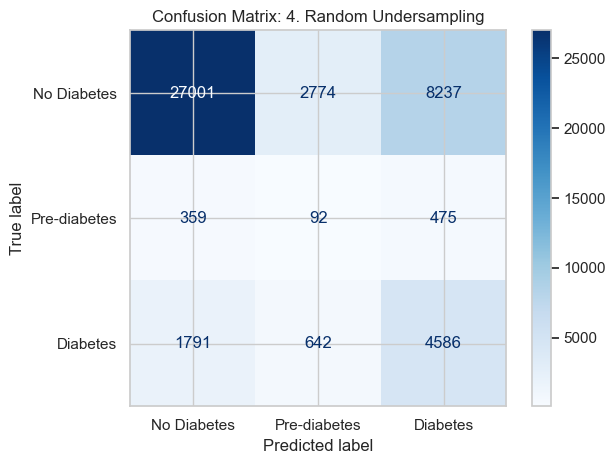
\includegraphics[width=0.45\textwidth]{softmax_undersampling_cm.png}
    \caption{Softmax Confusion Matrices: Baseline (top-left), SMOTE (top-right), Oversampling (bottom-left), Undersampling (bottom-right).}
\end{figure}

\begin{figure}[H]
    \centering
    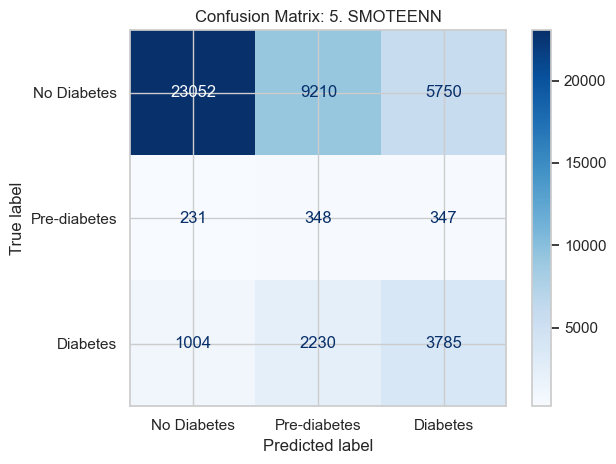
\includegraphics[width=0.45\textwidth]{softmax_smoteenn_cm.png}
    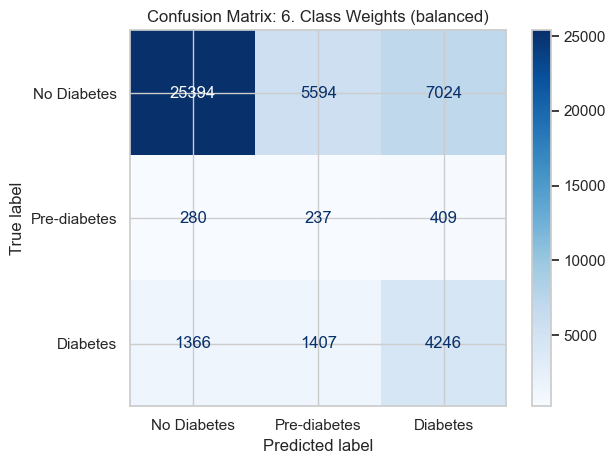
\includegraphics[width=0.45\textwidth]{softmax_classweights_cm.png} \\
    \vspace{0.3cm}
    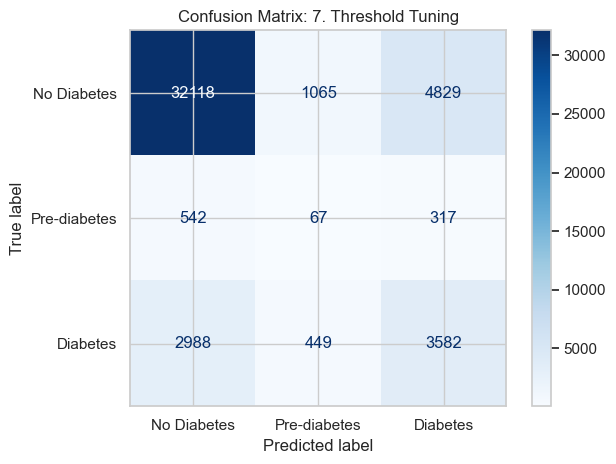
\includegraphics[width=0.45\textwidth]{softmax_thresholdtuning_cm.png}
    \caption{Softmax Confusion Matrices: SMOTEENN (top-left), Class Weights (top-right), Threshold Tuning (bottom-left).}
\end{figure}

\subsubsection{Feedforward Neural Network (FNN)}
\begin{figure}[H]
    \centering
    % \includegraphics[width=0.45\textwidth]{fnn_baseline_cm.png}
    % \includegraphics[width=0.45\textwidth]{fnn_smote_cm.png} \\
    \vspace{0.5cm}
    % \includegraphics[width=0.45\textwidth]{fnn_oversample_cm.png}
    % \includegraphics[width=0.45\textwidth]{fnn_undersample_cm.png}
    \caption{FNN Confusion Matrices (Top Left: Baseline, Top Right: SMOTE, Bottom Left: Oversampled, Bottom Right: Undersampled)}
\end{figure}

\section{Analysis and Comparison}

\subsection{Model Comparison}
Among the models evaluated so far, the Softmax Regression and KNN models show a clear trade-off between raw accuracy and Macro-F1. The Softmax Baseline achieves the highest accuracy (83.31\%) but a low Macro-F1 (0.3886), essentially predicting only the majority class. Once imbalance handling is applied, Softmax with Threshold Tuning achieves the best Macro-F1 among all Softmax variants (0.4602), outperforming SMOTE-based KNN (0.4166). This demonstrates that a linear model with proper calibration can exceed a distance-based model on this task.

For the FNN, the baseline model again achieves the highest accuracy (0.8380) but the lowest Macro-F1 (0.3915), confirming that accuracy is inflated by the dominant ``No Diabetes'' class. Once imbalance handling is introduced, the FNN variants converge to a tighter band of Macro-F1 scores, with the best result achieved by Random Undersampling (Macro-F1 = 0.4279). Class Weights (0.4243) yields a very similar performance without altering the dataset size, while SMOTE and Random Oversampling provide comparable improvements (0.4186 and 0.4194 respectively). SMOTEENN performs worst among the balancing strategies (0.4028), likely due to the combined over/under-sampling removing borderline samples that the network could otherwise learn from.

Overall, the FNN improves substantially over its own baseline when trained with imbalance-aware strategies, but it does not exceed the best calibrated linear approach (Softmax with threshold tuning, Macro-F1 = 0.4602). This suggests that, for this dataset, careful decision calibration and imbalance handling can be more impactful than model complexity.

The key insight is that Softmax Regression, being a linear model, is faster to train and tune across many strategies, while KNN is more sensitive to the local geometry of the feature space. Both models struggle significantly with the ``Prediabetes'' class due to its extreme rarity (only 2\% of samples). Threshold Tuning (best thresholds: [0.1, 0.3, 0.3]) partially addresses this by aggressively lowering the decision boundary for minority classes.

\subsection{Impact of Imbalance Handling}
Comparing the baseline models to the balanced models clearly demonstrates the necessity of handling class imbalance. For KNN, the baseline model achieved a high overall accuracy of 81.66\%, but suffered from a low Macro-F1 score of 0.3994, indicating it was heavily biased toward the majority class. Applying SMOTE reduced the overall accuracy to 71.77\% but successfully increased the Macro-F1 score to 0.4166. This shift proves that the balancing technique improved the model's ability to predict the difficult minority classes (like Prediabetes), making the classifier much more clinically useful despite the mathematical drop in raw accuracy.

\subsection{Insights and Misclassification Patterns}
Inspecting the confusion matrices for Softmax Regression reveals a consistent and clinically important pattern: the \textbf{``Prediabetes'' class is almost entirely misclassified as ``No Diabetes''} across all strategies. Even with aggressive balancing (SMOTE, Undersampling, Threshold Tuning), the model rarely correctly identifies a Prediabetes sample.

This occurs for two compounding reasons:
\begin{enumerate}
    \item \textbf{Mathematical:} The Prediabetes class represents only $\sim$2\% of the dataset. Even after balancing the training set, the decision boundary learned by a linear model is dominated by the much larger ``No Diabetes'' and ``Diabetes'' clusters. The Prediabetes feature distribution overlaps heavily with ``No Diabetes'', making it nearly impossible for a linear separator to isolate.
    \item \textbf{Clinical:} Prediabetes is, by definition, a borderline condition. Patients in this category share many health indicators with healthy individuals (normal BMI, moderate blood pressure), making the distinction genuinely ambiguous even for medical professionals. The features available in this dataset (binary lifestyle indicators) may not capture the subtle biochemical differences that distinguish Prediabetes from No Diabetes.
\end{enumerate}

The Threshold Tuning strategy partially addresses this by lowering the decision threshold for the Prediabetes class, allowing the model to ``bet'' on Prediabetes more aggressively. However, this comes at the cost of increased false positives for that class.

\section{Bonus: TensorBoard Monitoring}
During neural network training, TensorBoard was used to monitor convergence and generalisation by tracking both training and validation metrics per epoch. This is particularly important for this dataset because accuracy can look deceptively high due to the dominant ``No Diabetes'' class; therefore, the validation loss trend is a more reliable indicator of whether the network is learning a stable decision boundary.

\subsection{Training Dynamics (Loss and Accuracy Curves)}
Figures \ref{fig:tb_loss} and \ref{fig:tb_acc} show the epoch-level learning curves exported from TensorBoard.

\begin{figure}[H]
    \centering
    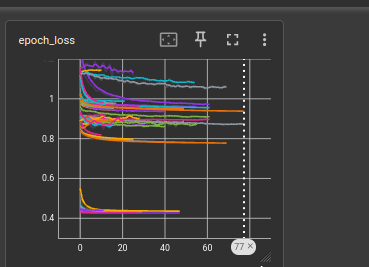
\includegraphics[width=0.7\textwidth]{epoch_loss.png}
    \caption{TensorBoard training and validation loss across epochs.}
    \label{fig:tb_loss}
\end{figure}

\begin{figure}[H]
    \centering
    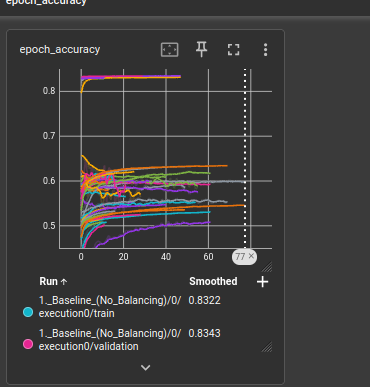
\includegraphics[width=0.7\textwidth]{epoch_accuracy.png}
    \caption{TensorBoard training and validation accuracy across epochs.}
    \label{fig:tb_acc}
\end{figure}

\subsection{Overfitting vs. Underfitting Diagnosis}
We interpret the curves using the following standard criteria:
\begin{itemize}
    \item \textbf{Good fit:} training loss decreases and validation loss decreases (or plateaus) with a small, stable gap.
    \item \textbf{Overfitting:} training loss continues decreasing while validation loss stops improving and begins increasing (a widening generalisation gap). This is often accompanied by training accuracy increasing while validation accuracy stagnates or drops.
    \item \textbf{Underfitting:} both training and validation losses remain high (or decrease very slowly), and accuracies remain low, indicating insufficient model capacity or excessive regularisation.
\end{itemize}

In our runs, the training loss decreases steadily while the validation loss improves early and then tends to plateau, with only a modest gap between the two curves. This pattern indicates \textbf{limited overfitting} rather than severe memorisation. The validation accuracy follows a similar behaviour, improving initially and then flattening, which suggests that the network reaches the limit of what can be learned from the available feature set.

Early stopping (monitoring validation loss) further reduces overfitting risk by restoring the best-performing weights from the point where validation performance peaks. Finally, the remaining discrepancy between training and validation metrics is consistent with the class-imbalance challenge and the difficulty of the minority ``Pre-diabetes'' class, for which the decision boundary is intrinsically noisy given the feature overlap with ``No Diabetes''.

\subsection{Optimisation Stability (Learning Rate and Internal Statistics)}
In addition to loss/accuracy, we exported supplementary TensorBoard plots that help diagnose optimisation stability:
\begin{itemize}
    \item \textbf{Learning Rate:} shows whether the optimiser is training with a constant step size or a schedule.
    \item \textbf{Bias and Beta:} internal parameter statistics from normalisation layers (e.g., BatchNorm), which indicate whether the network parameters are drifting smoothly or changing abruptly.
    \item \textbf{Moving Variance:} tracked by normalisation layers; instability (large oscillations) can indicate noisy gradients or an overly aggressive learning rate.
\end{itemize}

\begin{figure}[H]
    \centering
    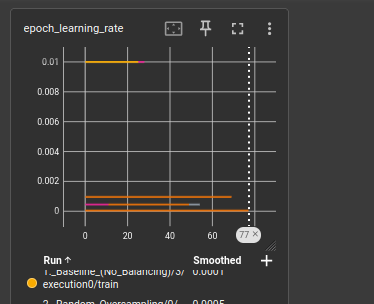
\includegraphics[width=0.75\textwidth]{learning_rate.png}
    \caption{Learning rate over training steps/epochs. A stable (or smoothly decaying) learning rate typically supports steady convergence, while abrupt jumps can correlate with spiky validation curves.}
\end{figure}

\begin{figure}[H]
    \centering
    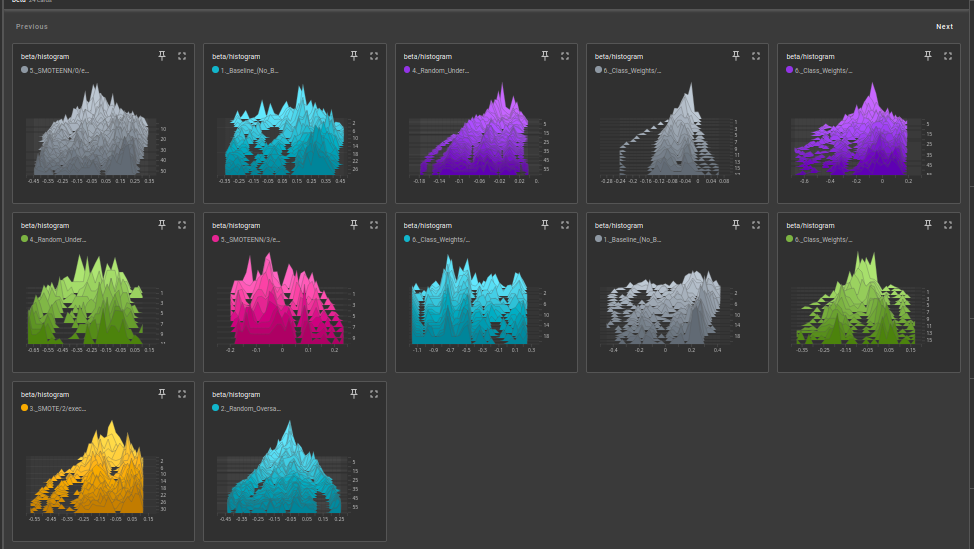
\includegraphics[width=0.85\textwidth]{beta.png}
    \caption{TensorBoard parameter trace (beta). Smooth trends suggest stable optimisation; sharp discontinuities would indicate unstable updates.}
\end{figure}

\begin{figure}[H]
    \centering
    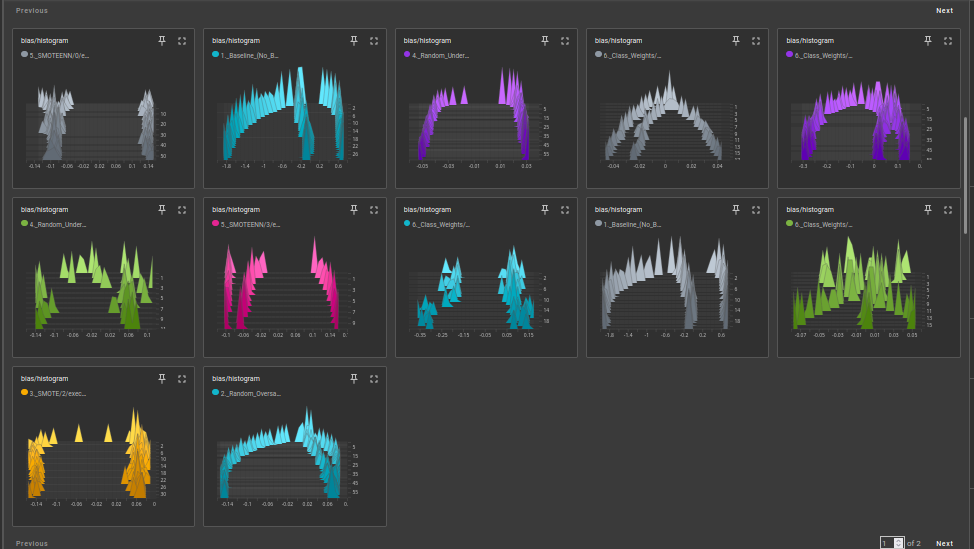
\includegraphics[width=0.85\textwidth]{bias.png}
    \caption{TensorBoard parameter trace (bias). When bias parameters grow rapidly while validation loss stops improving, it can be a sign of overfitting or poor calibration.}
\end{figure}

\begin{figure}[H]
    \centering
    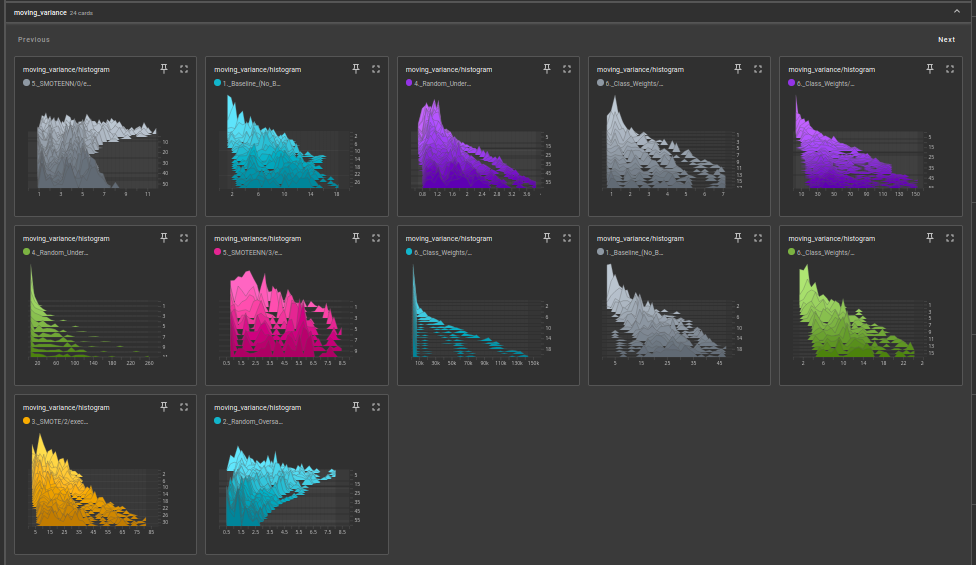
\includegraphics[width=0.85\textwidth]{moving_Variance.png}
    \caption{Moving variance trace from normalisation layers. Stable/slowly-changing variance indicates consistent feature scaling across batches; high oscillation can reflect gradient noise (often worse under heavy undersampling).}
\end{figure}

Overall, these diagnostic plots suggest that training was \textbf{numerically stable}: the learning dynamics evolve smoothly rather than exhibiting abrupt parameter jumps. This supports the conclusion from the loss curves that performance is limited primarily by the dataset difficulty and class overlap (especially for ``Pre-diabetes''), rather than by optimiser divergence.

\end{document}